\chapter{Experimental Setting}
\label{chapter:Experimental Setting}


\section{Meta-World Benchmark}
\label{section:Meta-World Benchmark}
To evaluate R-CIdL and compare its performance to the base method D-COACH, we use two simulated environments from the open-source benchmark Meta-World \cite{metaworld}. Meta-World 
provides 50 standardized manipulation tasks that use a simulated Sawyer arm. Even if this benchmark was specifically designed for multi-task and meta-reinforcement learning, it is possible to simply access single goal environments as we do in this thesis. All Meta-World tasks are implemented in the MuJoCo physics engine \cite{mujoco} and it is interfaced with OpenAI Gym \cite{openai} making it easy to use. 

\subsection{Meta-World: plate\_slide\_v2 task}
\label{subsection:metaworld-hockey-task}
Officially called plate\_slide\_v2 task

The closed end effector presses down the puck and slides it into the goal
First it has to go to the puck and then to the goal


$[\delta x, \delta y, \delta z, \text{gripper effort}]$

For each task, Meta-World includes an oracle policy

In order to evaluate the method along with subtle variants under more controlled conditions, a high performance policy standing-in as a teacher was used. The simulated teacher generates feedback computing $h = sign(a_\text{teacher} - a_\text{agent})$, whereas the decision on whether to provide feedback at each time step is given by the probability $P_h = \alpha \cdot exp(-\tau \cdot timestep)$, where $\{\alpha \in \mathbb{R}\, | 0 \leq \alpha \leq 1 \}$; $\{\tau \in \mathbb{R} \, | 0 \leq \tau\}$

 

 \begin{figure}[H]
  \centering
  \hspace*{\fill}%
  \subfloat[1 - Approach to puck]{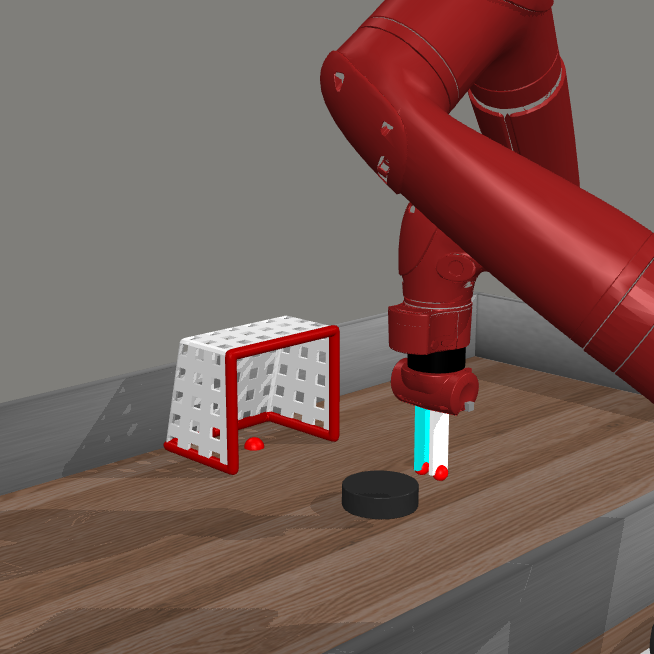
\includegraphics[width=0.28\textwidth]{figures/hockeypos0_v2.png}\label{fig:hockey_pos_0}}
   \hfill
  \subfloat[2 - Press puck vertically]{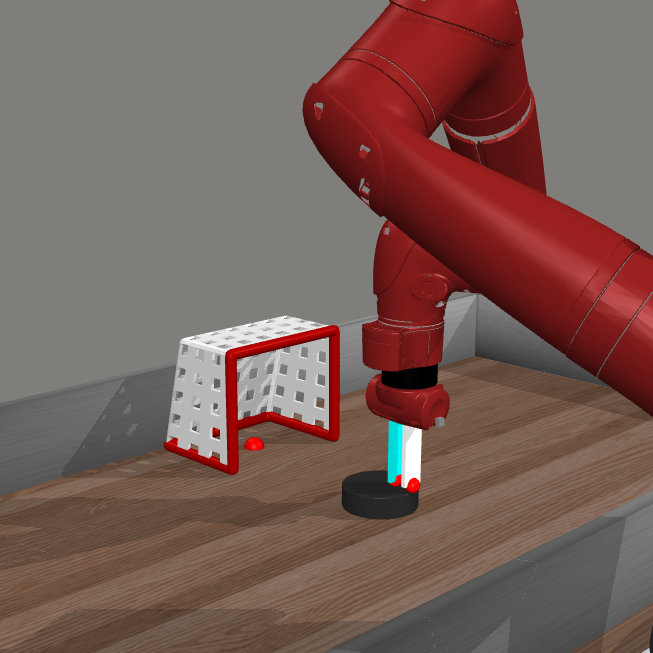
\includegraphics[width=0.28\textwidth]{figures/hockeypos1_v2.png}\label{fig:hockey_pos_1}}
   \hfill
  \subfloat[3 - Slide puck to goal]{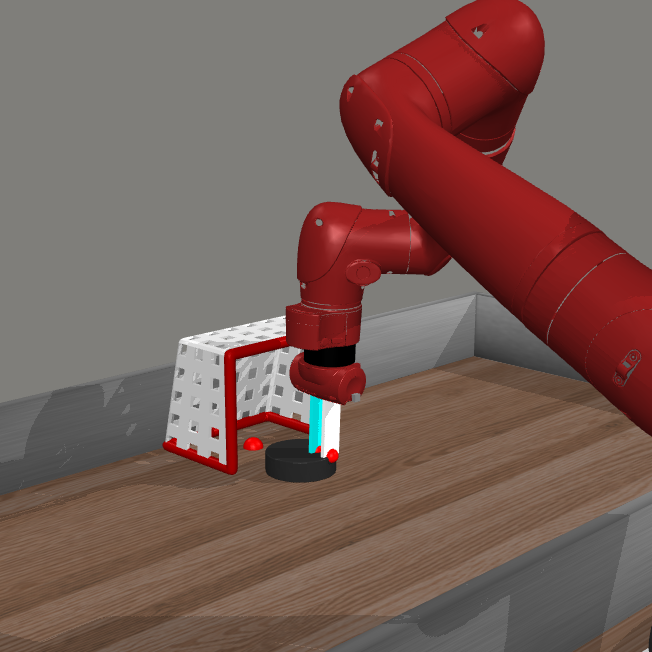
\includegraphics[width=0.28\textwidth]{figures/hockeypos2_v2.png}\label{fig:hockey_pos_2}}
  \hspace*{\fill}%
  \caption{Sequence of the plate\_slide\_v2 task in Meta-World}.
\end{figure}

\subsection{Meta-World: Open a drawer task}
\label{subsection:metaworld-open-drawer-task}



 \begin{figure}[H]
  \centering
  \hspace*{\fill}%
  \subfloat[1 - Approach to handle]{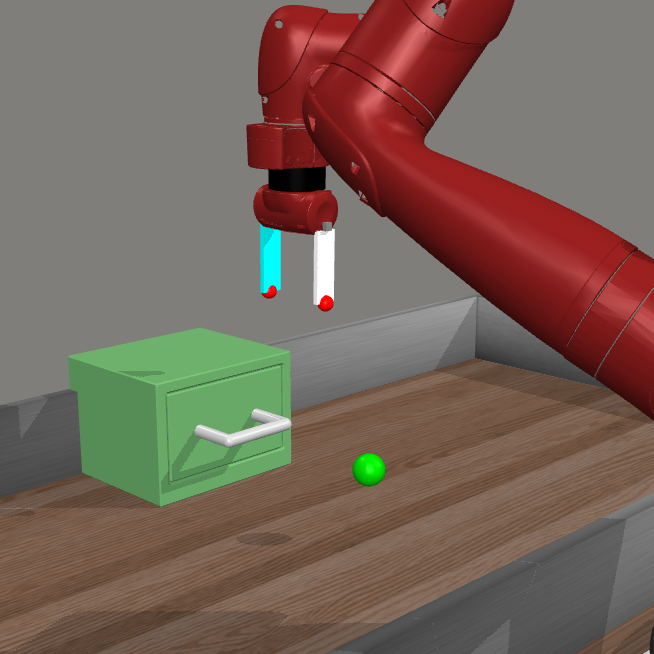
\includegraphics[width=0.28\textwidth]{figures/drawerpos0_v2.png}\label{fig:drawer_pos_0}}
   \hfill
  \subfloat[2 - Hook handle]{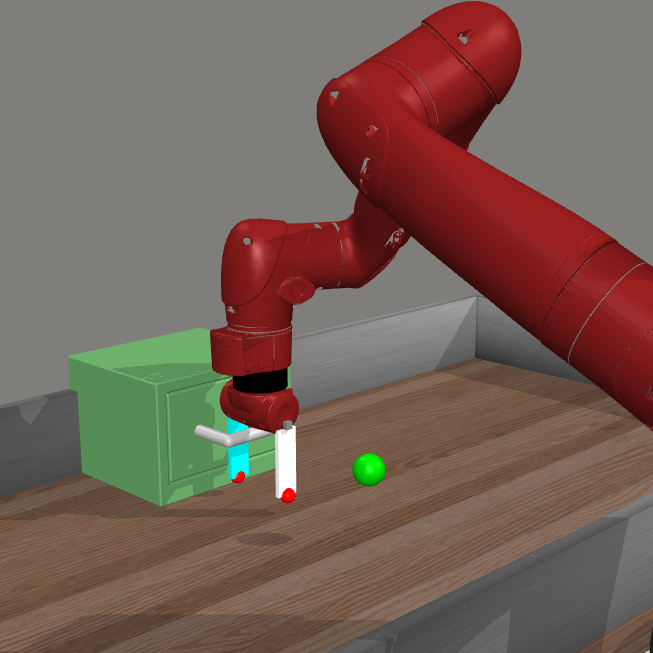
\includegraphics[width=0.28\textwidth]{figures/drawerpos1_v2.png}\label{fig:drawer_pos_1}}
   \hfill
  \subfloat[3 - Open drawer]{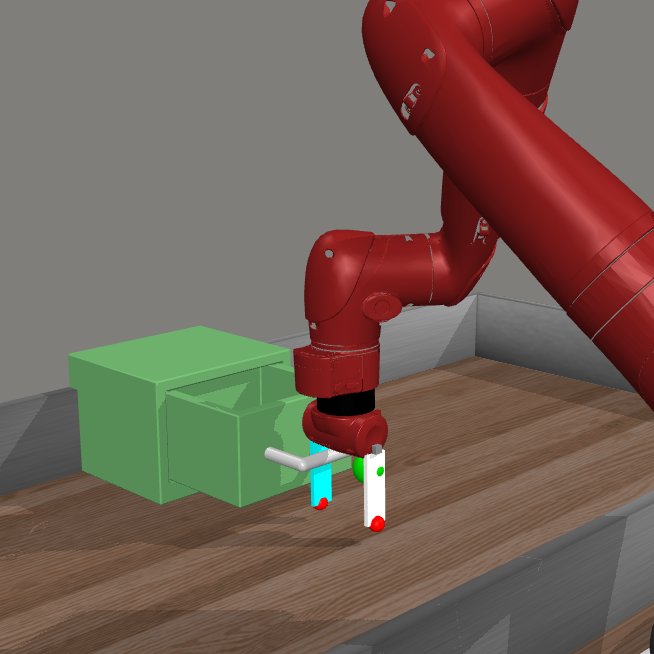
\includegraphics[width=0.28\textwidth]{figures/drawerpos2_v2.png}
  \label{fig:drawer_pos_2}}
  \hspace*{\fill}%
  \caption{Sequence of the drawer\_open\_v2 task in Meta-World}.
\end{figure}


drawer\_open\_v2

Open end effector. The drawer is initiated closed, first it hooks the handle of the drawer and then it retracts to open it.

timestep = 
%max_path_length = 500
success metric
random init
after every 5 training episodes
75000 timesteps which correspond to blabla simulated minutes.

Table \ref{tab:hyperparameters} shows the parameters used for the experiments.



\begin{table}[H]
\centering
\renewcommand{\arraystretch}{1.4}
\begin{tabular}{llS[table-format=2.2]SSS[table-format=2.2]S[table-format=2.2]}
\toprule
\textbf{Parameter }& \textbf{Value}\\[-.4em]
\midrule
Policy hidden sizes  &   (256, 128)\\
Policy activation of hidden layers  &   (tanh, tanh)\\
Policy learning rate  &  0.001\\
Human model hidden sizes &   (512, 512)\\
Human model activation of hidden layers  &   (tanh, tanh)\\
Human model learning rate  &   0.001\\
Buffer sampling rate&   10\\
Buffer sampling size &   20\\
Time steps per training &   75000\\
Max time steps per episode &   500\\
\bottomrule
\end{tabular}
\caption{Hyperparameters used for the experiments}
\label{tab:hyperparameters}
\end{table}

Imagenes de dos puntos de la tarea enganche/tiron y busco puck/meto gol

quiza una vista de alzado para mostrar las random init pos


\section{Experiments with KUKA robot arm}
\label{section:Experiments with KUKA robot arm}

In order to validate the new proposed method RCIdL on a real robotic setup, we devised two tasks involving a KUKA LBR iiwa 7 robot arm pushing a box placed on top of a table; These 2 tasks will be explained later in more detail.

Several reflecting markers were attached to the box so its pose could be tracked by an OptiTrack motion capture system. The pose captured by the 8 cameras of the available OptiTrack system, consists on the position and orientation of the center point on the box created by the reflecting markers. 

The human that supervises the learning process conveys the corrections with a joystick. In order to make the task easier to teach, the human provides corrections just in the 2 axis parallel to the surface of the table while, the vertical position of the end effector is kept constant and close to the surface of the table . Prior to perform the real experiments, everything was checked in a simulated Gazebo environment.

A ROS network connects all the required elements for the experiment, these being: The feedback corrections from the joystick, the pose of the box from the optitrack and the position of the end effector of the KUKA. Specifically, for retrieving the position and sending the commands to the robot arm, the iiwa ROS stack \cite{iiwa} is used. 

For the control of the arm, the CustomControllers is used. It allows the control of the end effector in the cartesian space. Its command is formed by 6 values. The first 3 values are the orientation of the end effector ant the last 3, its position. For our purposes, we fix the orientation and the position in the vertical axis ~~and we command the x and y~~

The requested command in the remaining 2 positions is the current position of the end effector plus a delta which is the output of the network. Therefore the action the neural network of the agent outputs is a 2 dimensional representing thethat relative changes to the positions 

Regarding the state that enters to the policy, it has 7 dimensions these being:

- The relative position between the end effector and the box in the x axis (length of table axis)
- The relative position between the end effector and the box in the z axis (width of table axis)
- velocity of the end effector in the x axis
- velocity of the end effector in the z axis
- position of the box in the x axis
- position of the box in the z axis (from optitrack)
- pitch angle of the box (perpendicular to the surface of the table)

Finally, a binary metric of success was implemented. This metric has a value of 1 if the box ends within a small radius from the target position and 0 otherwise.

\subsection{Real task 1: Push a box in a straight line}

\label{subsection:Push box in a straight line}

The first task consist on a box placed at a side of the table and the goal is that the kuka has to push it until a target position (indicated with a green cross). Even if it looks like a simple, as \cite{constant_velocity} Planar manipulation problem, where the goal is to control the motion of an object, the slider, using a robotic pusher. It is an unstable system, lets say the goal is to push an object in a straight line with a pushing interaction, but if you don't have a reactive robot, you just can't do this task, the robot will naturally fall outside. This task really highlights the importance of feedback control and reactive robots

.. isn't as trivial as it looks like. Figure \ref{fig:planar-motion-problem} shows this problem. A constant velocity is commanded to the end effector. Because the robot doesn't react to small misalignments, the box keeps deviation from the  desired straight trajectory.


 \begin{figure}[H]
  \centering
  \hspace*{\fill}%
  \subfloat{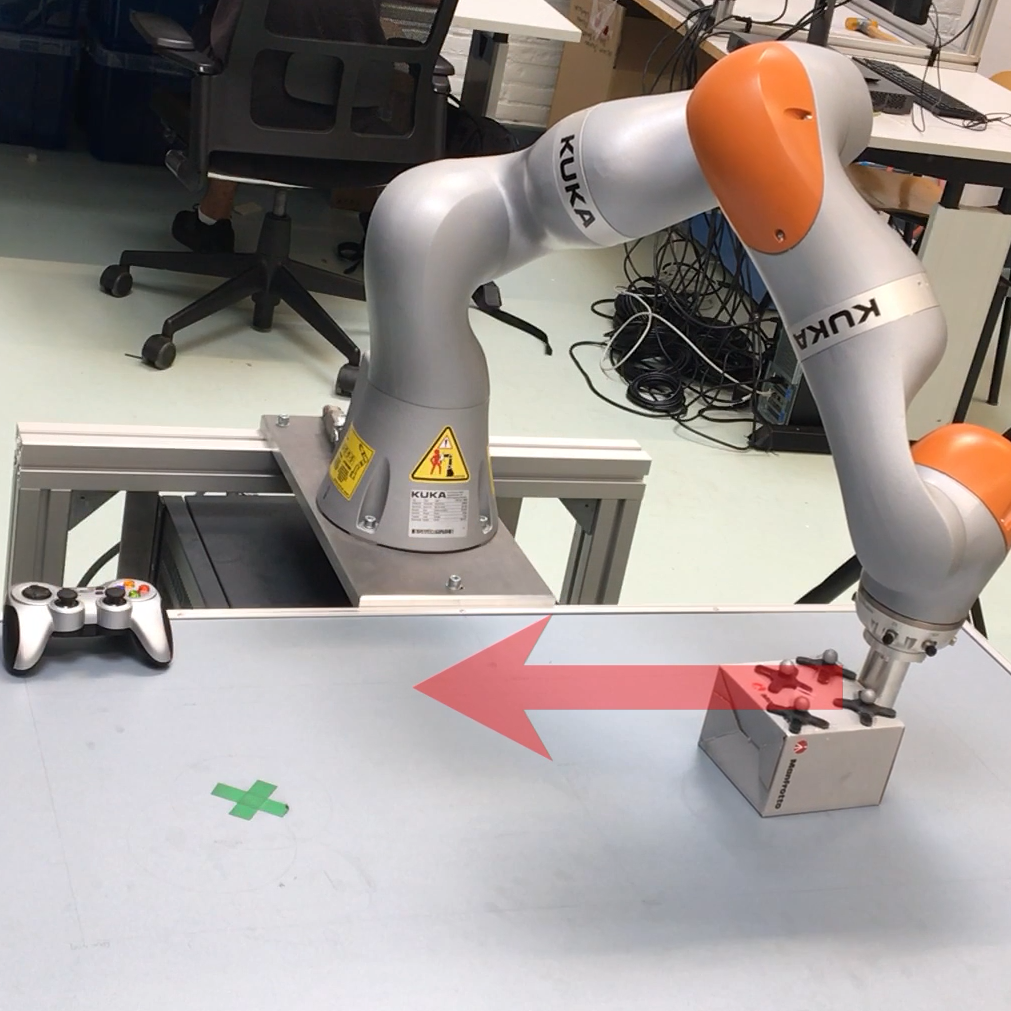
\includegraphics[width=0.25\textwidth]{figures/const_vel0.png}\label{fig:drawer_pos_0}}
   \hfill
  \subfloat{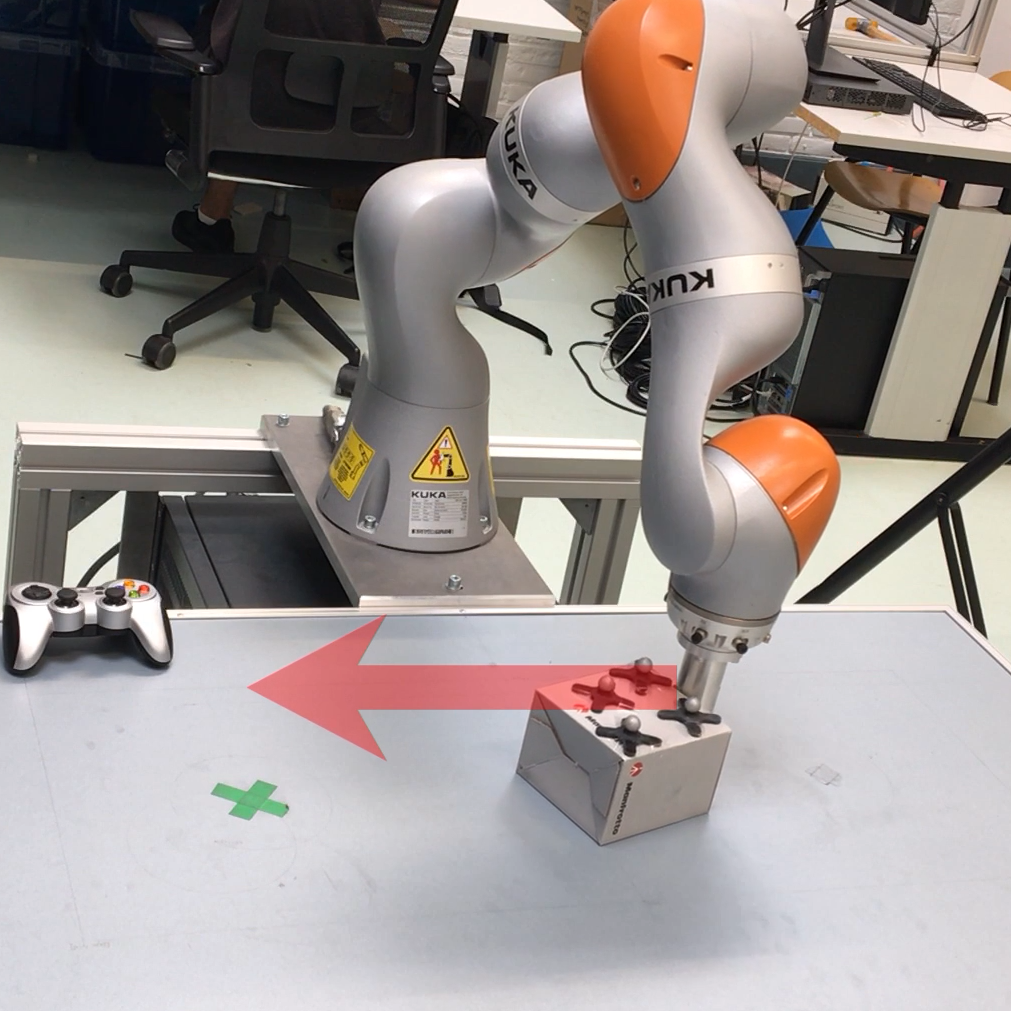
\includegraphics[width=0.25\textwidth]{figures/const_vel1.png}\label{fig:drawer_pos_1}}
   \hfill
  \subfloat{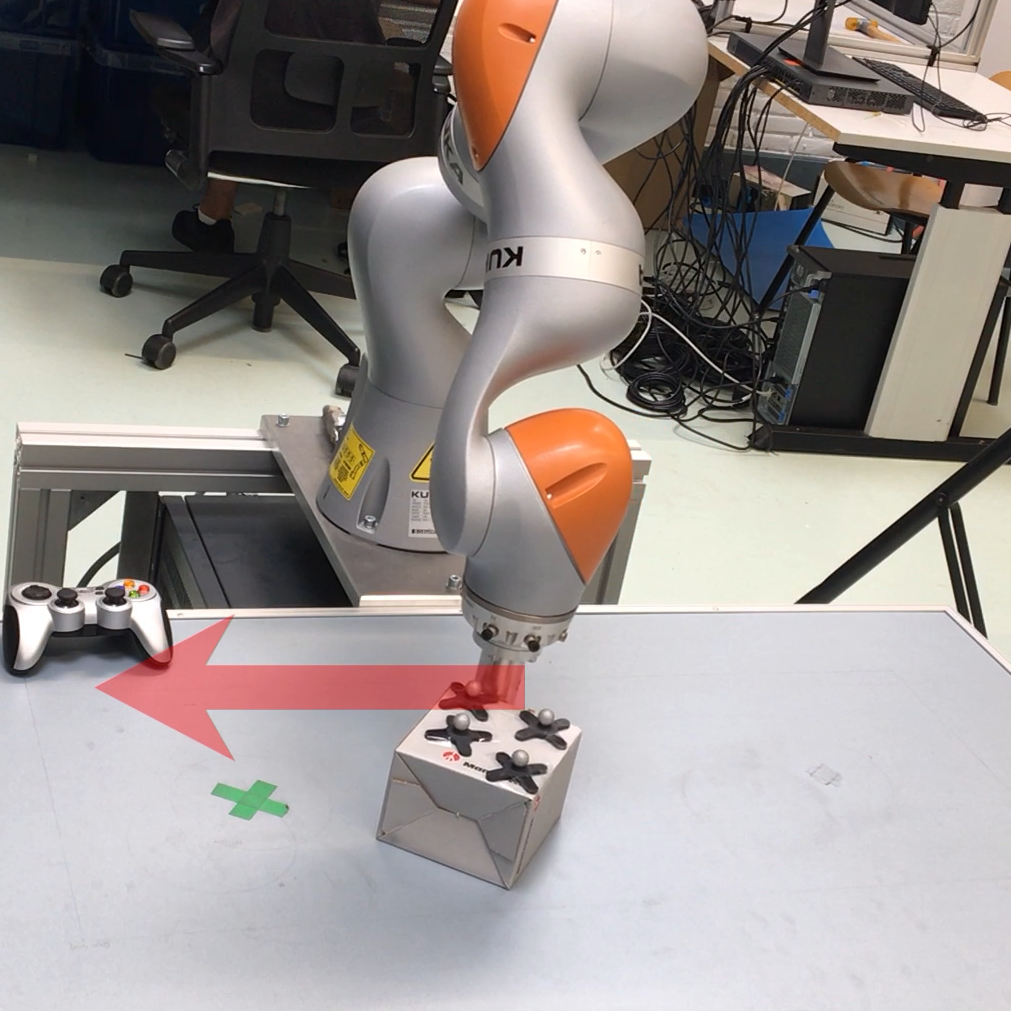
\includegraphics[width=0.25\textwidth]{figures/const_vel2.png}\label{fig:drawer_pos_2}}
   \hspace*{\fill}%
  \caption{By applying a constant velocity, the box gets easily misaligned.}
  \label{fig:planar-motion-problem}
\end{figure}

Figure \ref{fig:push-box} shows a sequence of the task once the agent has been trained using R-CIdL. The box is initialized in random positions and disturbances are manually introduced. The agent is able to succesfully reach the goal by learning to continuous back and forth motion to quickly correct the misalignments of the box.

 \begin{figure}[H]
  \centering
  \subfloat[1 - Start position]{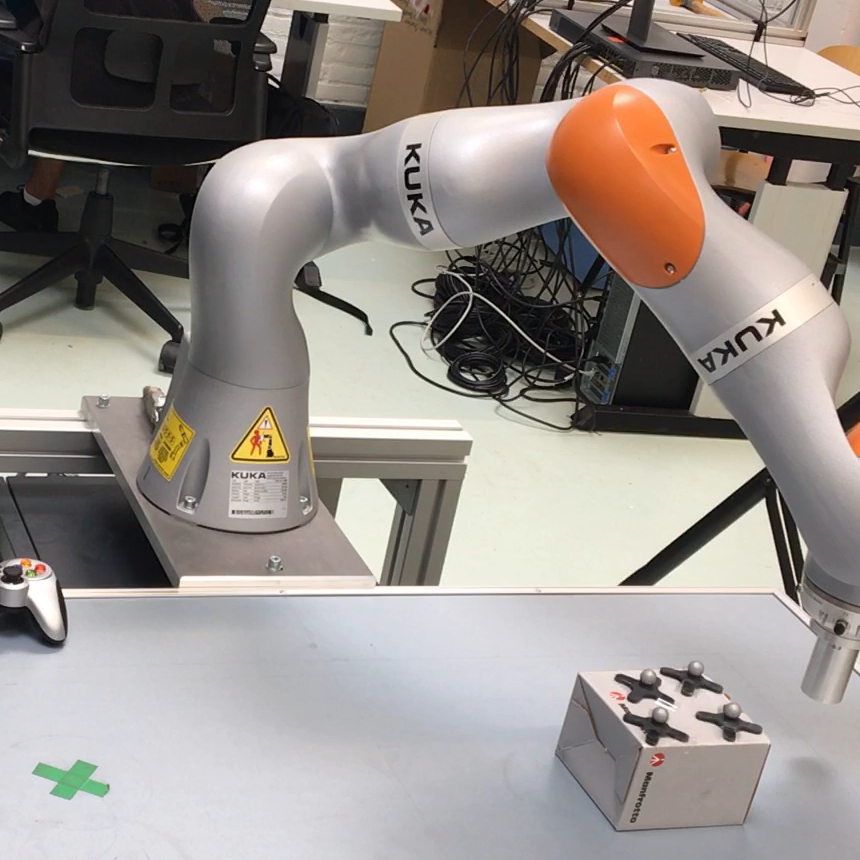
\includegraphics[width=0.19\textwidth]{figures/push0.png}\label{fig:push_pos_0}}
   \hfill
  \subfloat[2 - Approach to box]{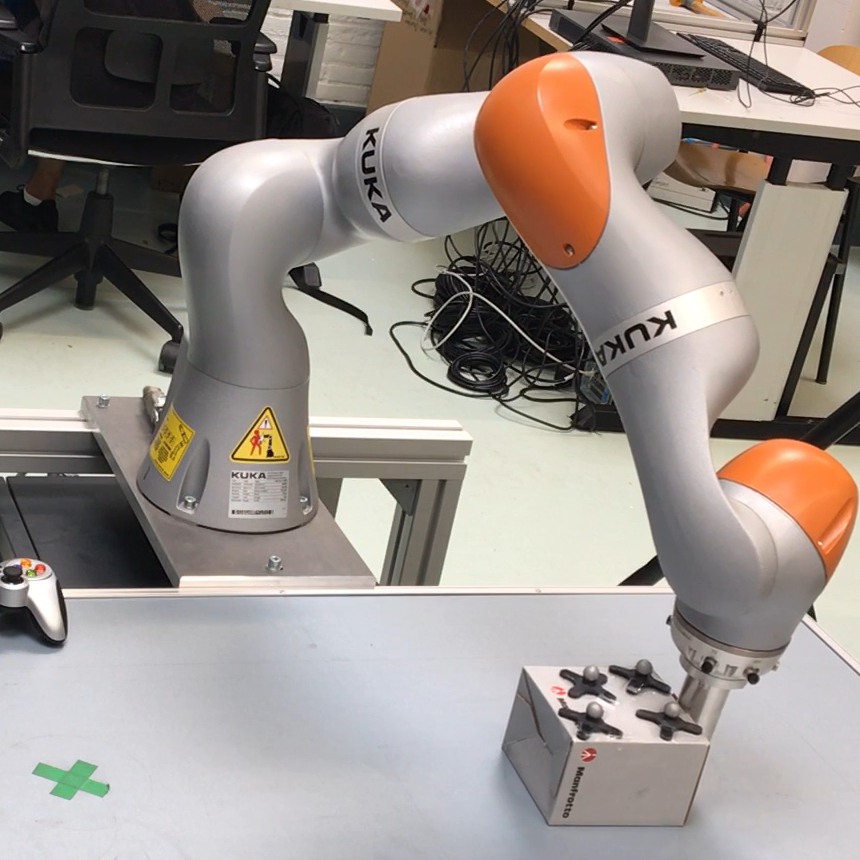
\includegraphics[width=0.19\textwidth]{figures/push1.png}\label{fig:push_pos_1}}
   \hfill
  \subfloat[3 - Introduce disturbance]{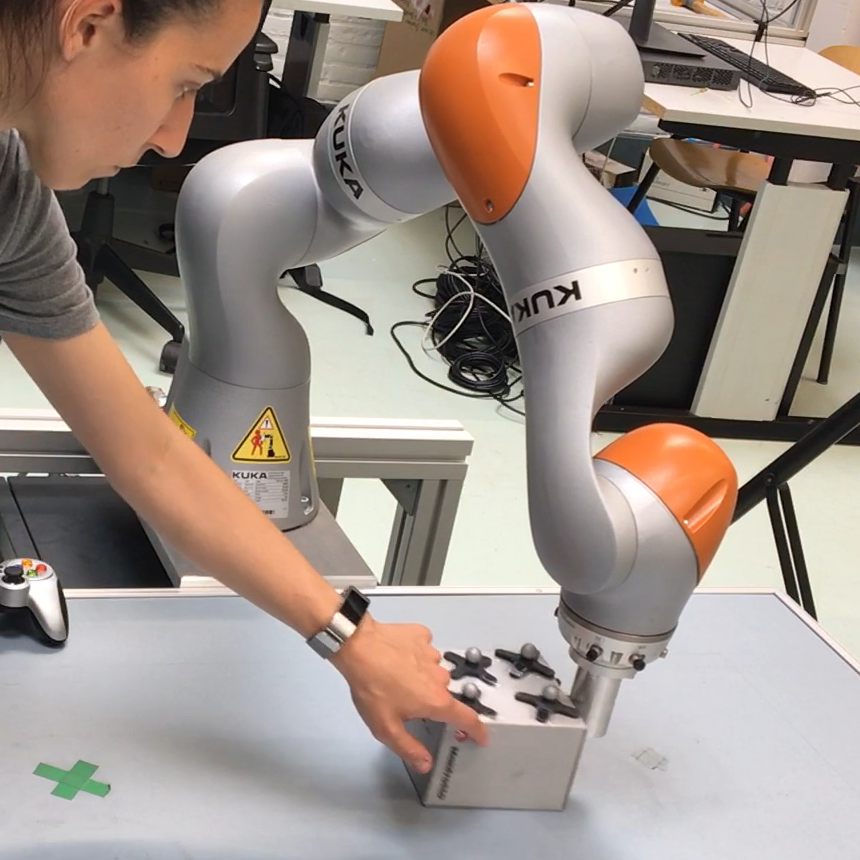
\includegraphics[width=0.19\textwidth]{figures/push2.png}\label{fig:push_pos_2}}
   \hfill
  \subfloat[4 - Correct disturbance]{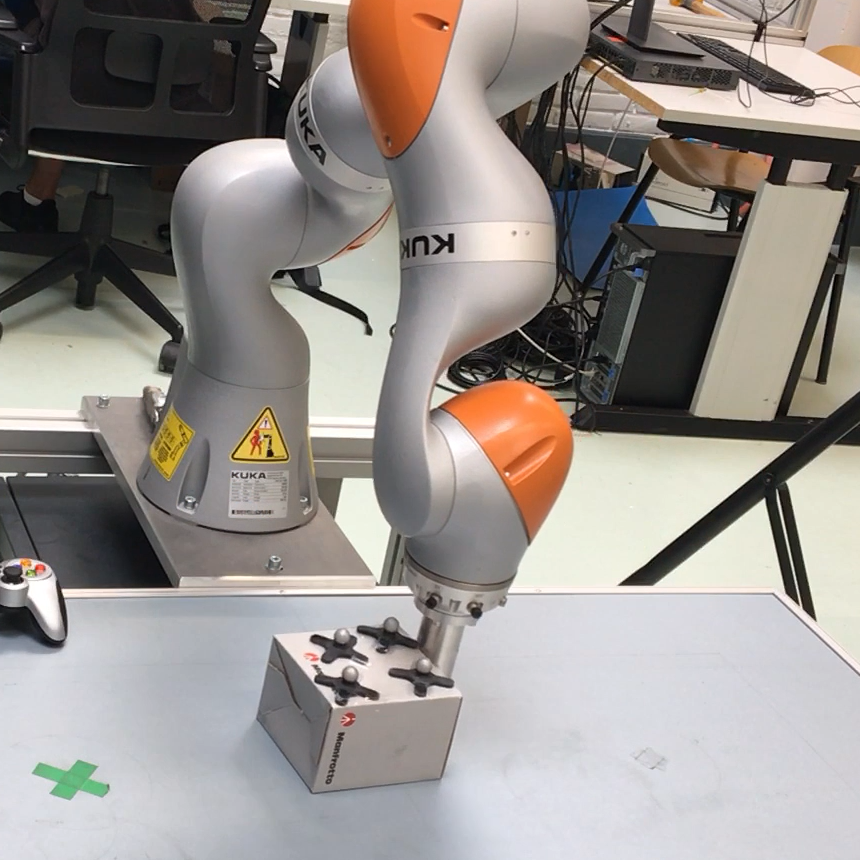
\includegraphics[width=0.19\textwidth]{figures/push3.png}\label{fig:push_pos_2}}
   \hfill
  \subfloat[5 - End position]{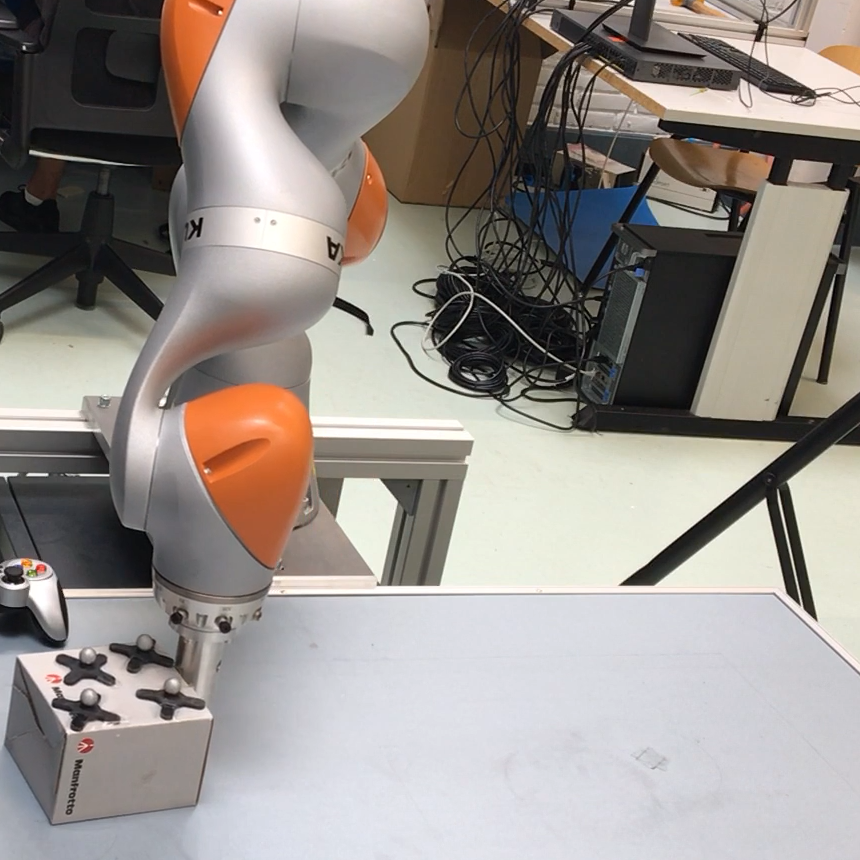
\includegraphics[width=0.19\textwidth]{figures/push5.png}\label{fig:push_pos_2}}
  \caption{Sequence of the task "push a box"}.
  \label{fig:push-box}
\end{figure}







\subsection{KUKA task 2: Park a box}
\label{subsection:Park a box}

The second task also involves pushing a box but this time the sequence of movements is more complex. The goal is in both axis parallel to the surface of the table. Once it has pushed it and center it until it faces the 2 brown boxes, the end effector moves around the corner of the box and starts pushing from the other side until it is fit between the 2 walls. 

Figure \ref{fig:park-box} shows the sequence of movements for this task.


 \begin{figure}[H]
  \centering
  \subfloat[1 - Start position]{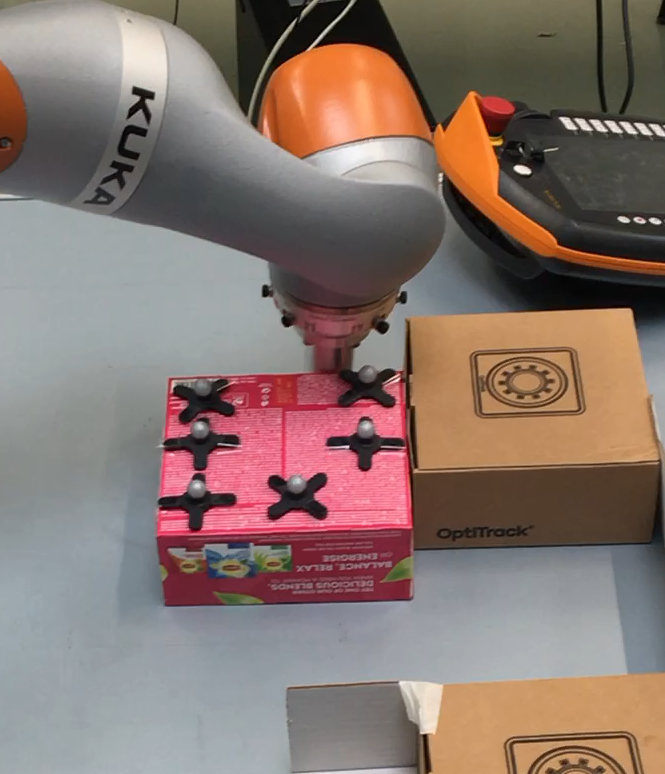
\includegraphics[width=0.16\textwidth]{figures/park0_v2.png}\label{fig:drawer_pos_0}}
   \hfill
  \subfloat[2 - Push box]{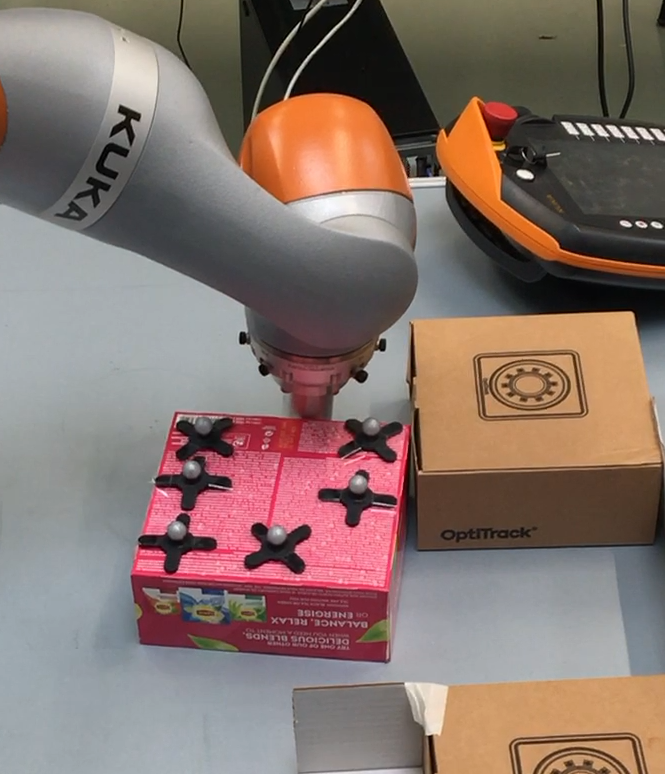
\includegraphics[width=0.16\textwidth]{figures/park1_v2.png}\label{fig:drawer_pos_1}}
   \hfill
  \subfloat[3 - Center box]{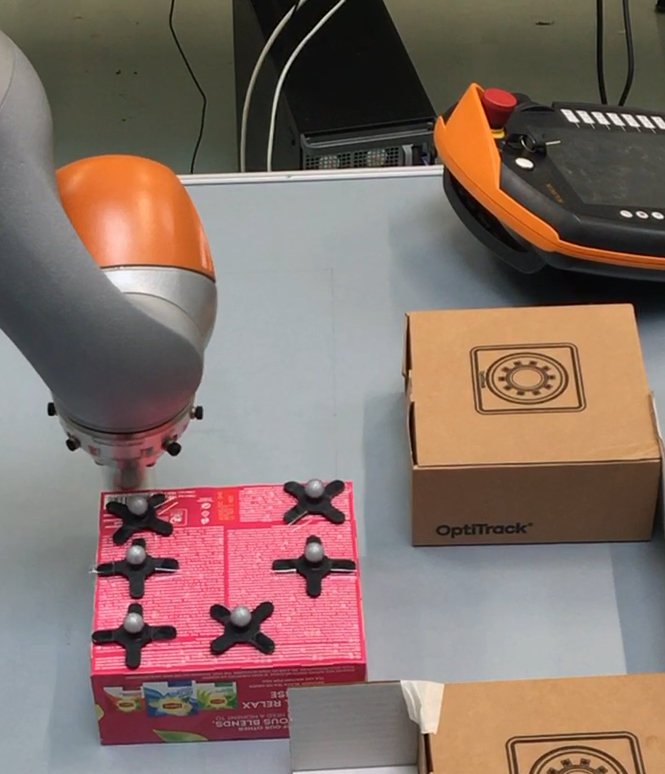
\includegraphics[width=0.16\textwidth]{figures/park3_v2.png}\label{fig:drawer_pos_2}}
   \hfill
  \subfloat[4 - Move around corner]{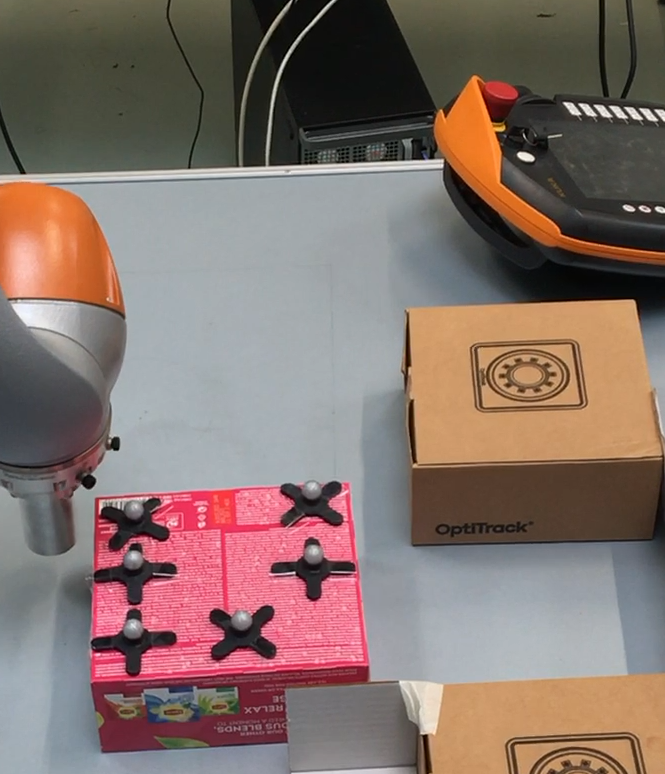
\includegraphics[width=0.16\textwidth]{figures/park4_v2.png}\label{fig:drawer_pos_2}}
   \hfill
  \subfloat[5- Push box between walls]{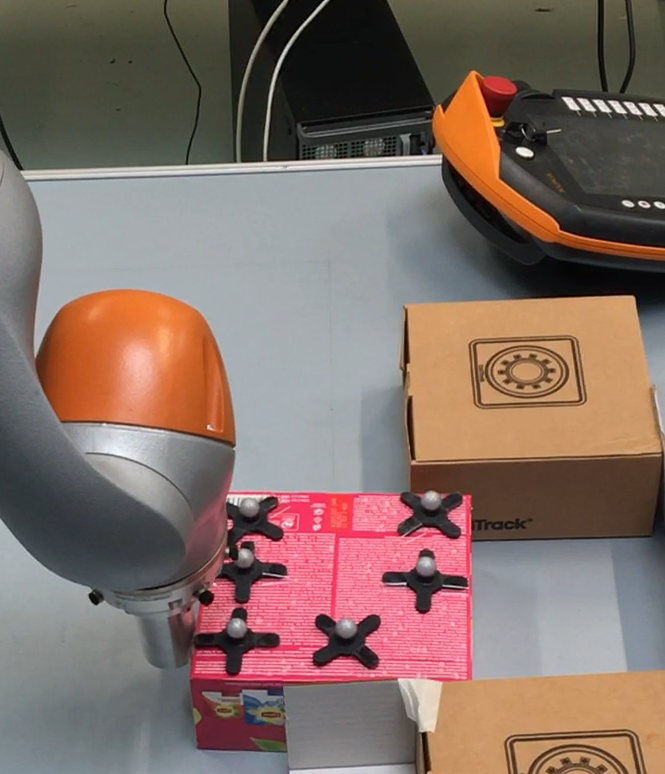
\includegraphics[width=0.16\textwidth]{figures/park5_v2.png}\label{fig:drawer_pos_2}}
   \hfill
  \subfloat[6 - End position]{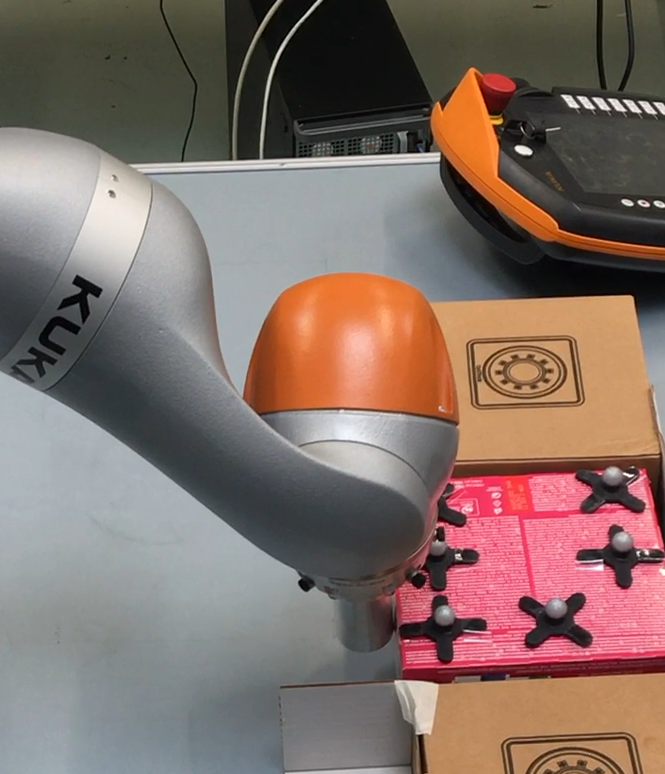
\includegraphics[width=0.16\textwidth]{figures/park6_v2.png}\label{fig:drawer_pos_2}}
  \caption{Sequence of the task "park a box"}.
  \label{fig:park-box}
\end{figure}

